\subsection{Plots}\label{subsec:plots}
	
\begin{figure}[H]
\begin{center}
%Here begins the 3d plot
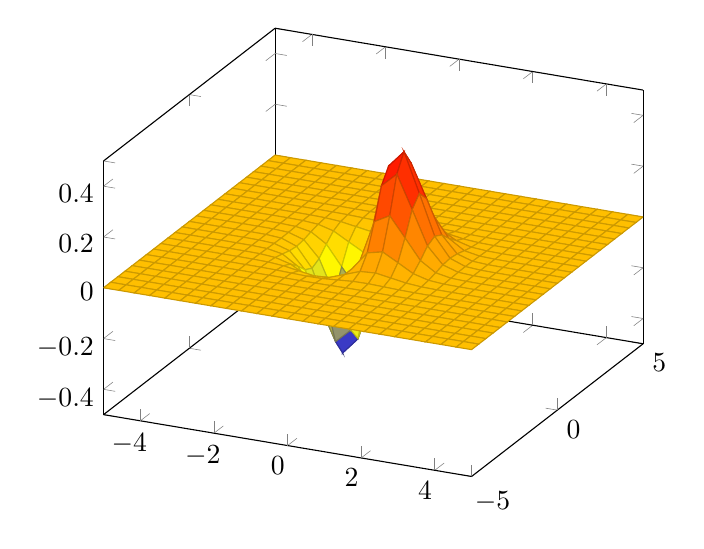
\begin{tikzpicture}
\begin{axis}
\addplot3[
    surf,
]
{exp(-x^2-y^2)*x};
\end{axis}
\end{tikzpicture}
\end{center}
\caption{Eigens erstellter Plot mit dem Paket libz und pgfplots}
\end{figure}


\begin{figure}[H]
\begin{center}
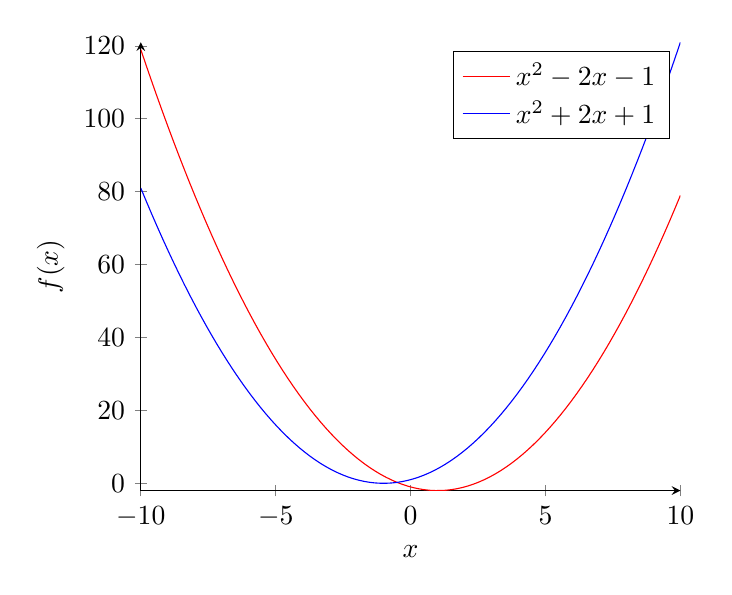
\begin{tikzpicture}
\begin{axis}[
    axis lines = left,
    xlabel = $x$,
    ylabel = {$f(x)$},
]
%Below the red parabola is defined
\addplot [
    domain=-10:10, 
    samples=100, 
    color=red,
]
{x^2 - 2*x - 1};
\addlegendentry{$x^2 - 2x - 1$}
%Here the blue parabloa is defined
\addplot [
    domain=-10:10, 
    samples=100, 
    color=blue,
    ]
    {x^2 + 2*x + 1};
\addlegendentry{$x^2 + 2x + 1$}

\end{axis}
\end{tikzpicture}
\end{center}
\caption{Eigens erstellter Plot mit dem Paket libz und pgfplots}
\end{figure}